\chapter{Data Acquisition, Audit and Curation}
\section{Provenance and integrity}
Kvasir~v2 (8{,}000 JPEG frames, 8 classes $\times$ 1{,}000) and Kvasir-SEG (1{,}000 polyp frames with expert masks) were downloaded from the owners'
server (\texttt{datasets.simula.no}) on 2 November 2026. The Kvasir~v2 archive is 2{,}489{,}312{,}085 bytes, equal to the server's reported
\texttt{Content-Length}; it passes Python's \texttt{zipfile.testzip()} and its SHA-256 is recorded in \texttt{data/raw/MANIFEST.json}. Extraction goes into an
empty directory and rejects absolute paths and \texttt{..} components, because archives are untrusted input.

\paragraph{An incident worth recording.} The first transfer silently stopped at 771\,MB: the server closed the connection and the shell pipeline hid
\texttt{curl}'s non-zero exit status. The size check caught it, and the final downloader (\texttt{data/download.py}) resumes with HTTP Range requests until the
byte count matches exactly.

\section{Defects discovered}
\begin{table}[h]
\centering\small
\caption{Data defects found in Kvasir~v2 and the action taken.}
\begin{tabular}{p{0.05\linewidth}p{0.42\linewidth}p{0.4\linewidth}}
\toprule
\# & Finding & Action \\
\midrule
1 & One file is byte-identical in two different classes (\texttt{dyed-lifted-polyps} and \texttt{dyed-resection-margins}) & both copies dropped \\
2 & 11 more byte-identical pairs; embedding duplicates (cosine $\ge 0.98$) bring the total to 30 pairs & first kept; \nDropped{} rows removed, \nClean{} remain \\
3 & Native resolution leaks the label: colon classes are 97--100\,\% 720$\times$576, upper-GI classes 90--97\,\% larger formats & FOV crop and square resize; leak measured at \resOnlyAcc{} (majority \regionMajority) \\
4 & ScopeGuide picture-in-picture box in \tealCecum{} of cecum frames, about 52\,\% of polyp frames, none of the upper-GI frames & canonical rectangle masked in \emph{every} frame \\
5 & First version of the box detector also hid blue dye (a lesion cue) & stricter colour, flatness and placement test; re-verified visually \\
6 & Burned-in overlay text; no EXIF personal-data fields in any file (0/8{,}000) & reported as a limitation \\
7 & No patient or video identifiers & scene groups from embedding similarity ($\ge 0.92$) \\
8 & Perceptual hashing fails: the shared octagonal border dominates low-frequency bits (at Hamming $\le 2$, 63 of 134 pairs were cross-class) & pHash only for exact matches \\
9 & Confident learning flags \nFlagged{} labels (\flaggedPct{}), concentrated in esophagitis, z-line and the two dyed classes & flagged, not removed \\
\bottomrule
\end{tabular}
\end{table}

\begin{figure}[h]
\centering
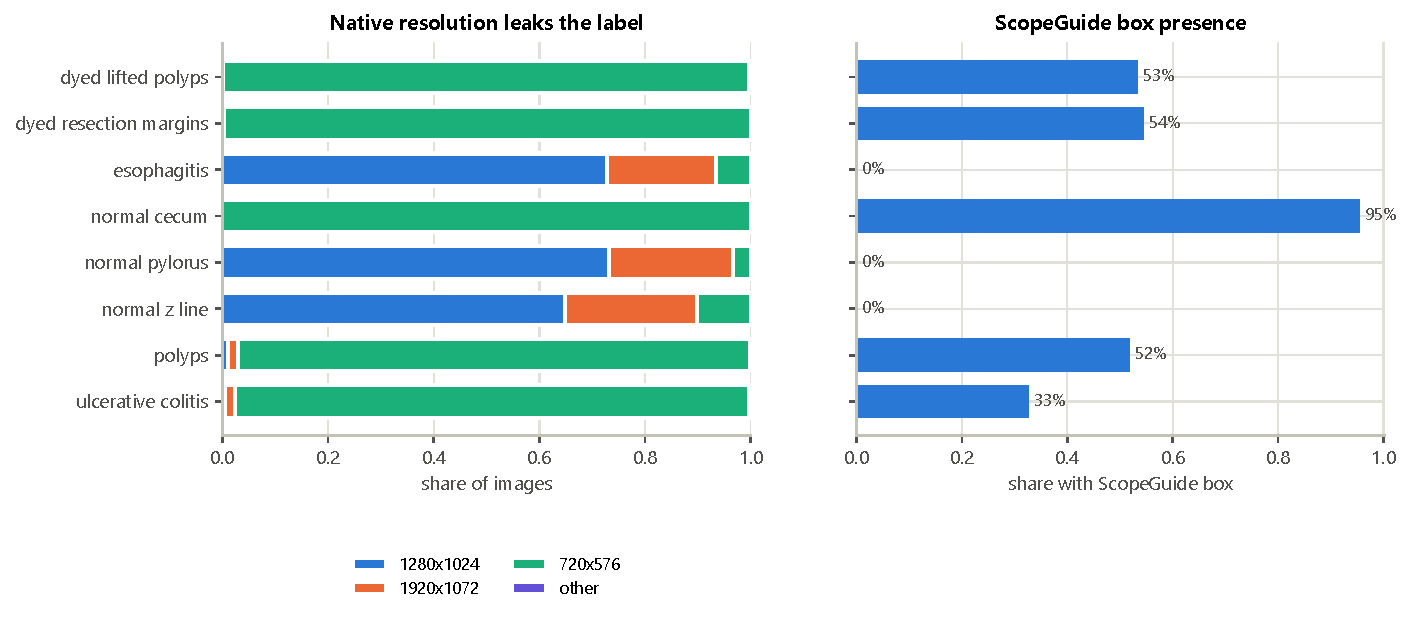
\includegraphics[width=0.95\linewidth]{eda_artefacts.pdf}
\caption{Acquisition artefacts by class: native-resolution mix (left) and presence of the ScopeGuide box (right).}
\end{figure}
\begin{figure}[h]
\centering
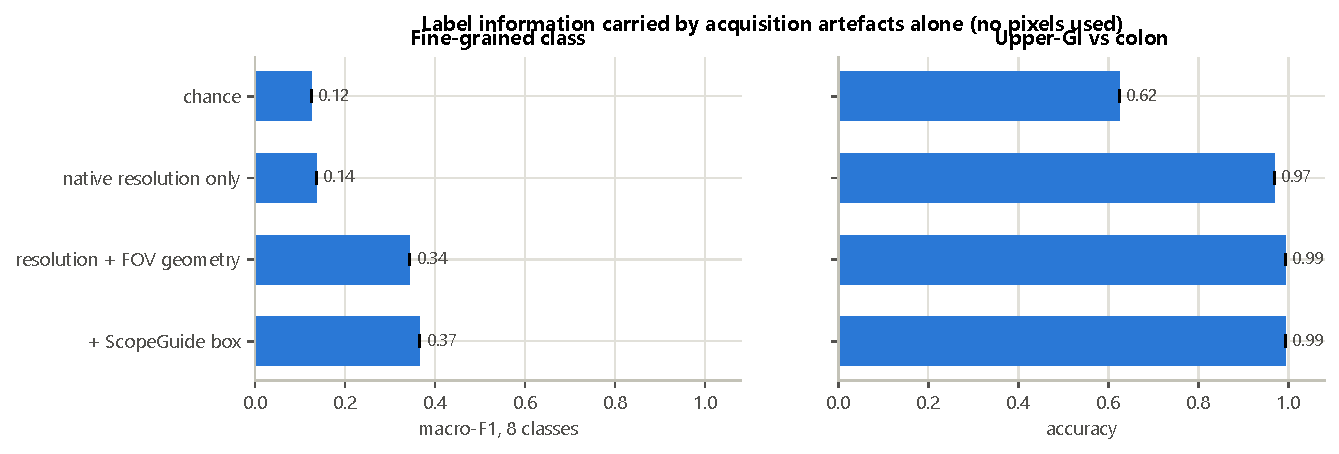
\includegraphics[width=0.8\linewidth]{eda_shortcut_probe.pdf}
\caption{Label information available from acquisition artefacts alone, using no pixel values. A gradient-boosted classifier on native resolution separates
upper-GI from colon frames with \resOnlyAcc{} accuracy, and with FOV geometry \resGeomAcc{}.}
\end{figure}

\section{Canonicalisation}
The endoscopic field of view is the largest bright blob after morphological opening (which strips thin text strokes); its convex hull gives the FOV
mask and the crop box. A rectangle covering the ScopeGuide location (measured on 419 detected boxes) is blacked out in every frame, and the \emph{valid}
mask excludes FOV exterior and this rectangle. Figure~\ref{fig:pipeline} shows the stages on three frames.

\begin{figure*}[t]
\centering
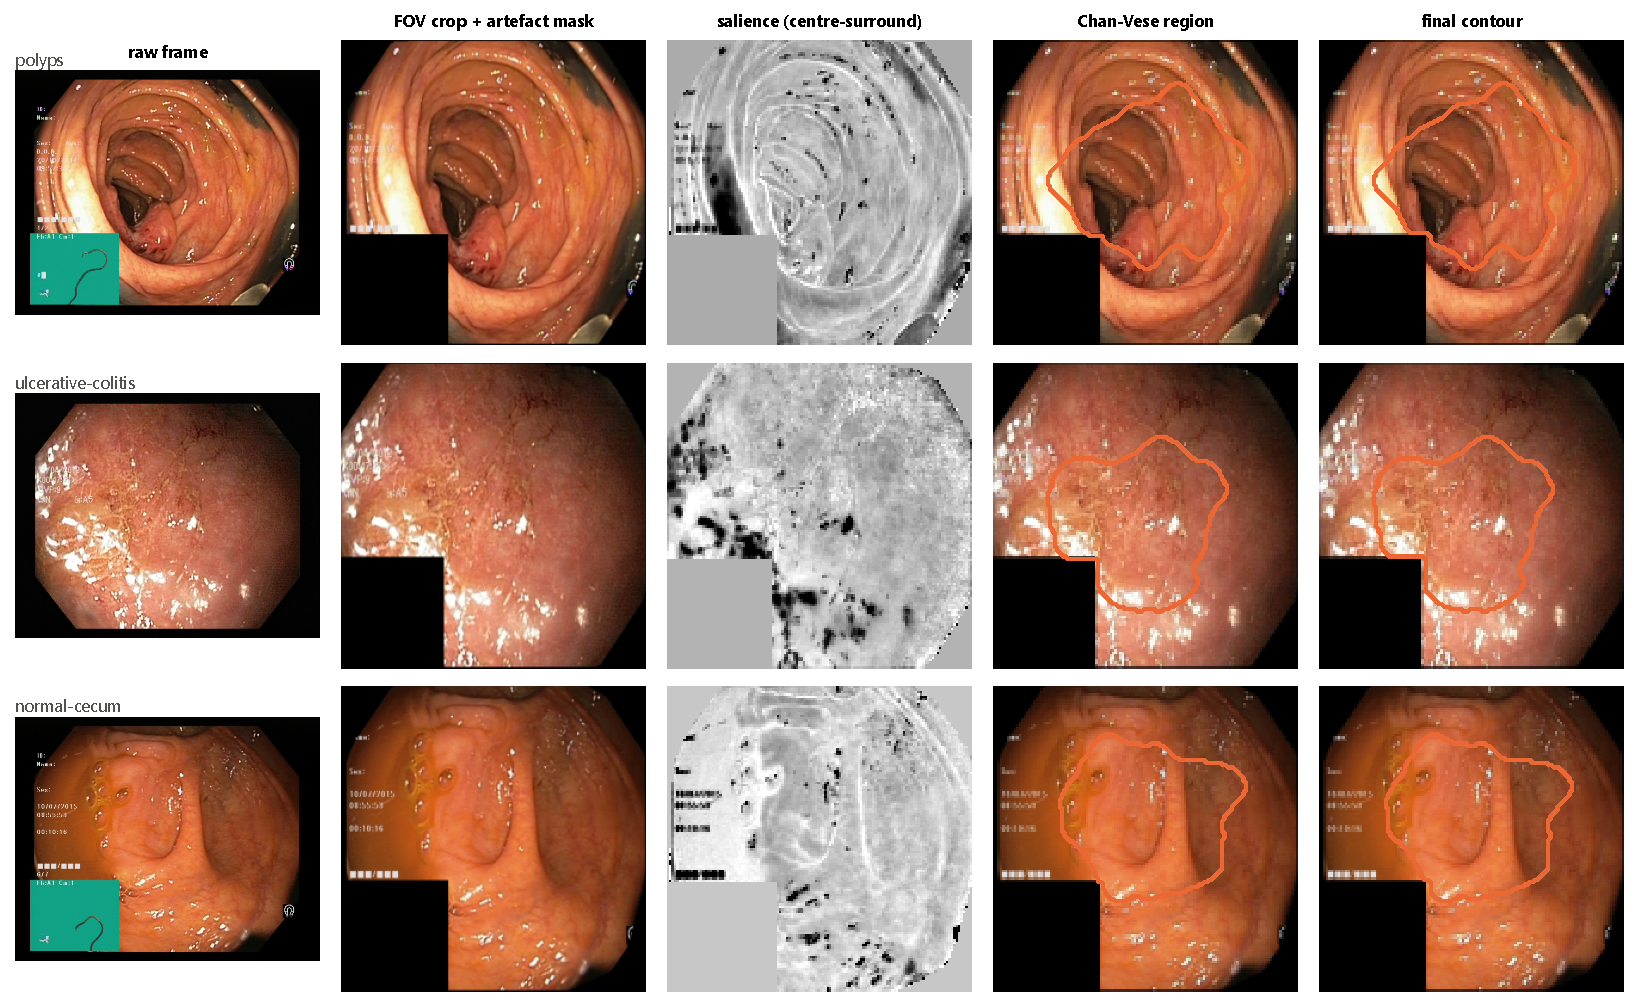
\includegraphics[width=0.9\linewidth]{ac_pipeline.pdf}
\caption{Pipeline illustration on a polyp, a colitis and a cecum frame: raw frame, FOV crop with artefact mask, centre--surround salience map, Chan--Vese region and final contour.}
\label{fig:pipeline}
\end{figure*}

\section{De-duplication, scene groups and splits}
Frozen DINOv2-S/14 embeddings give cosine similarity. Inspection of sampled pairs showed that similarity $\ge 0.95$ is the same frame, while 0.88--0.95
is the same lesion or lumen from a slightly different pose (consecutive frames of one procedure). Single-linkage at 0.90 chains into a 546-image blob, so the
group threshold is 0.92, giving \nGroups{} groups (largest 7). A stratified group split yields 5{,}578 / 797 / 1{,}594 train / val / test images with zero
group or hash overlap. A naive stratified random split with the same sizes would put \randLeakGroups{} groups on both sides of train/test; \randLeakPct{}
of its test images have a twin in the training set at similarity $\ge 0.92$. Near-duplicate leakage is therefore modest, and we report that size honestly.

\section{Distributions and collinearity}
Mean luma is close to normal (Shapiro--Wilk $p=0.16$), Laplacian variance is right-skewed (skew 1.36) and used on a log scale. The 98 contour-derived
features are heavily collinear (median VIF \vifMedian{}, \nVifTen{} features with VIF above 10), so regularised linear models and trees are used and
individual coefficients are never interpreted.

\begin{figure}[h]
\centering
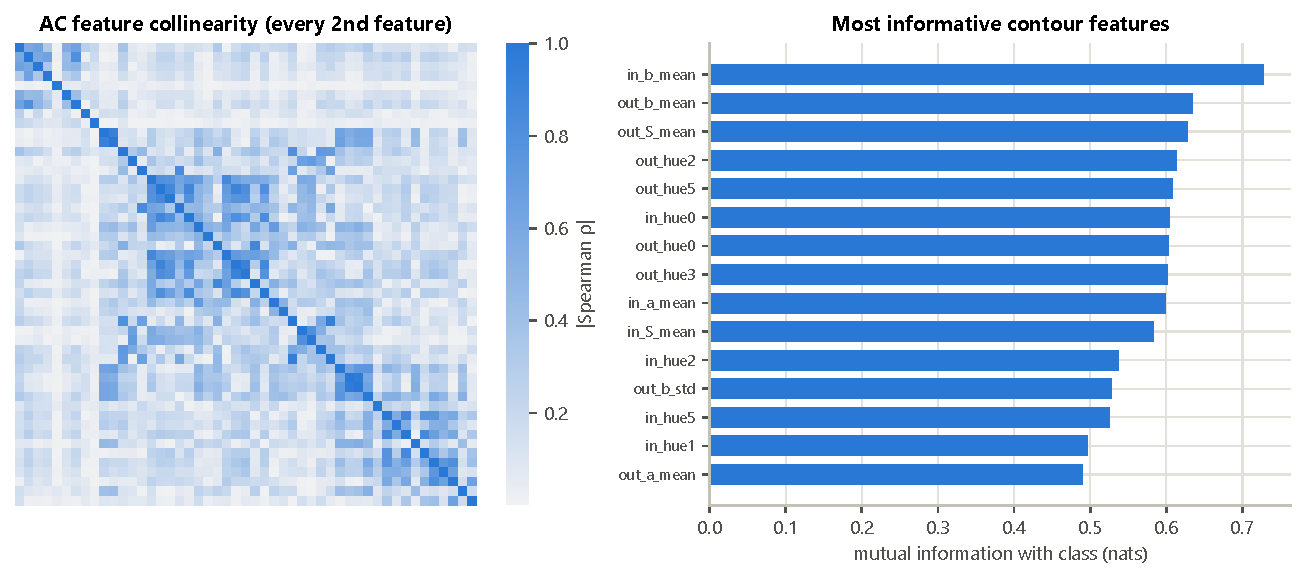
\includegraphics[width=0.95\linewidth]{eda_features.pdf}
\caption{Left: collinearity of the contour features. Right: mutual information of the most informative features with the class.}
\end{figure}
\begin{figure}[h]
\centering
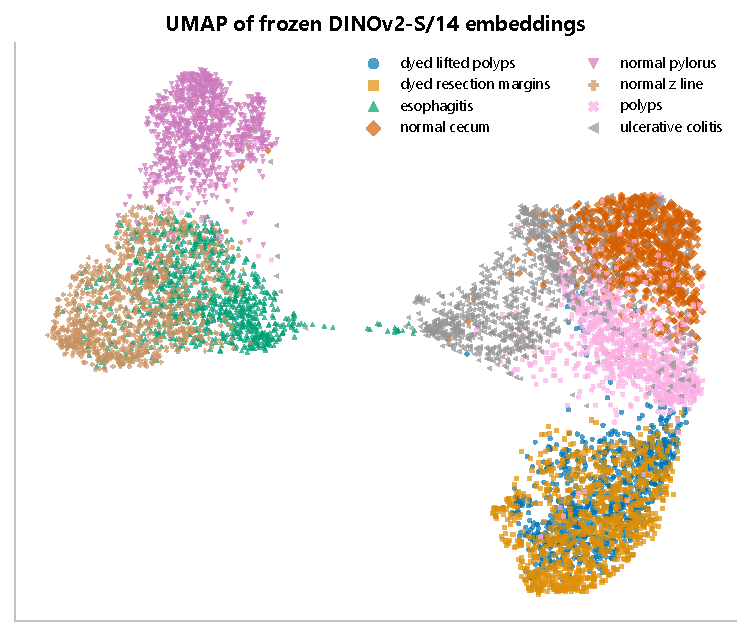
\includegraphics[width=0.6\linewidth]{eda_umap.pdf}
\caption{UMAP of frozen DINOv2 embeddings coloured by class (distinct marker shapes as a second channel).}
\end{figure}
